\chapter{Frozen Showers}\label{chap:FS}

As it was mentioned in a previous chapter, fast simulation techniques are the essential part of Monte-Carlo production at \atlas experiment. Typical time for a simulation of 1 $t\bar{t}$ event is around 1 minute, and most of the time is spend on a simulation of particle interaction in calorimeters. This is a main motivation of development of fast calorimetry techniques. 
Frozen showers is currently the main fast calorimeter simulation approach used at \atlas experiment. In this chapter we will discuss main principles and current developments in optimization of this method.

Frozen shower method uses pre-simulated "frozen" showers instead of the full simulation. This is allowing to reduce time spend on a simulation of a large amount of low energy sub showers. Typical number of frozen showers used in a simulation of 1 ttbar event is. This method is allowing to have a 25\% speedup. 

This method requiring in advance generation of a libraries for each detector and particle used in this method. Later, during fast simulation, if a particle energy falls below a cutoff it is replaced by a shower from a library. Main parameters used in \atlas simulation are summarized in a Tab. ~\ref{tab:MC_FS_params}. 

\begin{table}[b]
\caption{Main parameters used for the frozen shower libraries in FCAL }
\label{tab:MC_FS_params}
\centering
\begin{tabular}{l|r}
\hline
\hline
\multicolumn{2}{c}{The general frozen showers parameters} \\
\hline
Detectors used            & FCAL1, FCAL2\\
Type of the particle      & photons, electrons, neutrons \\
Energy range              &  $E_{\gamma}<10$~MeV,  $E_{e}<1000$~MeV,  $T_n<100$~MeV \\
Containment requirement   & $\Delta E_{shower} > 98\%$\\
\hline
\multicolumn{2}{c}{The library post-processing parameters} \\
\hline
Generation clustering cutoff & $(\Delta R_{cluster})^{2} < 25$ mm\\
Generation truncation cutoff & $R_{hit}^{2} < 50000$ mm, $\Delta E_{shower} < 1\%$\\
\hline
\hline
\end{tabular}

\end{table}

\section{Problem description}

\begin{figure}[!b]
\center{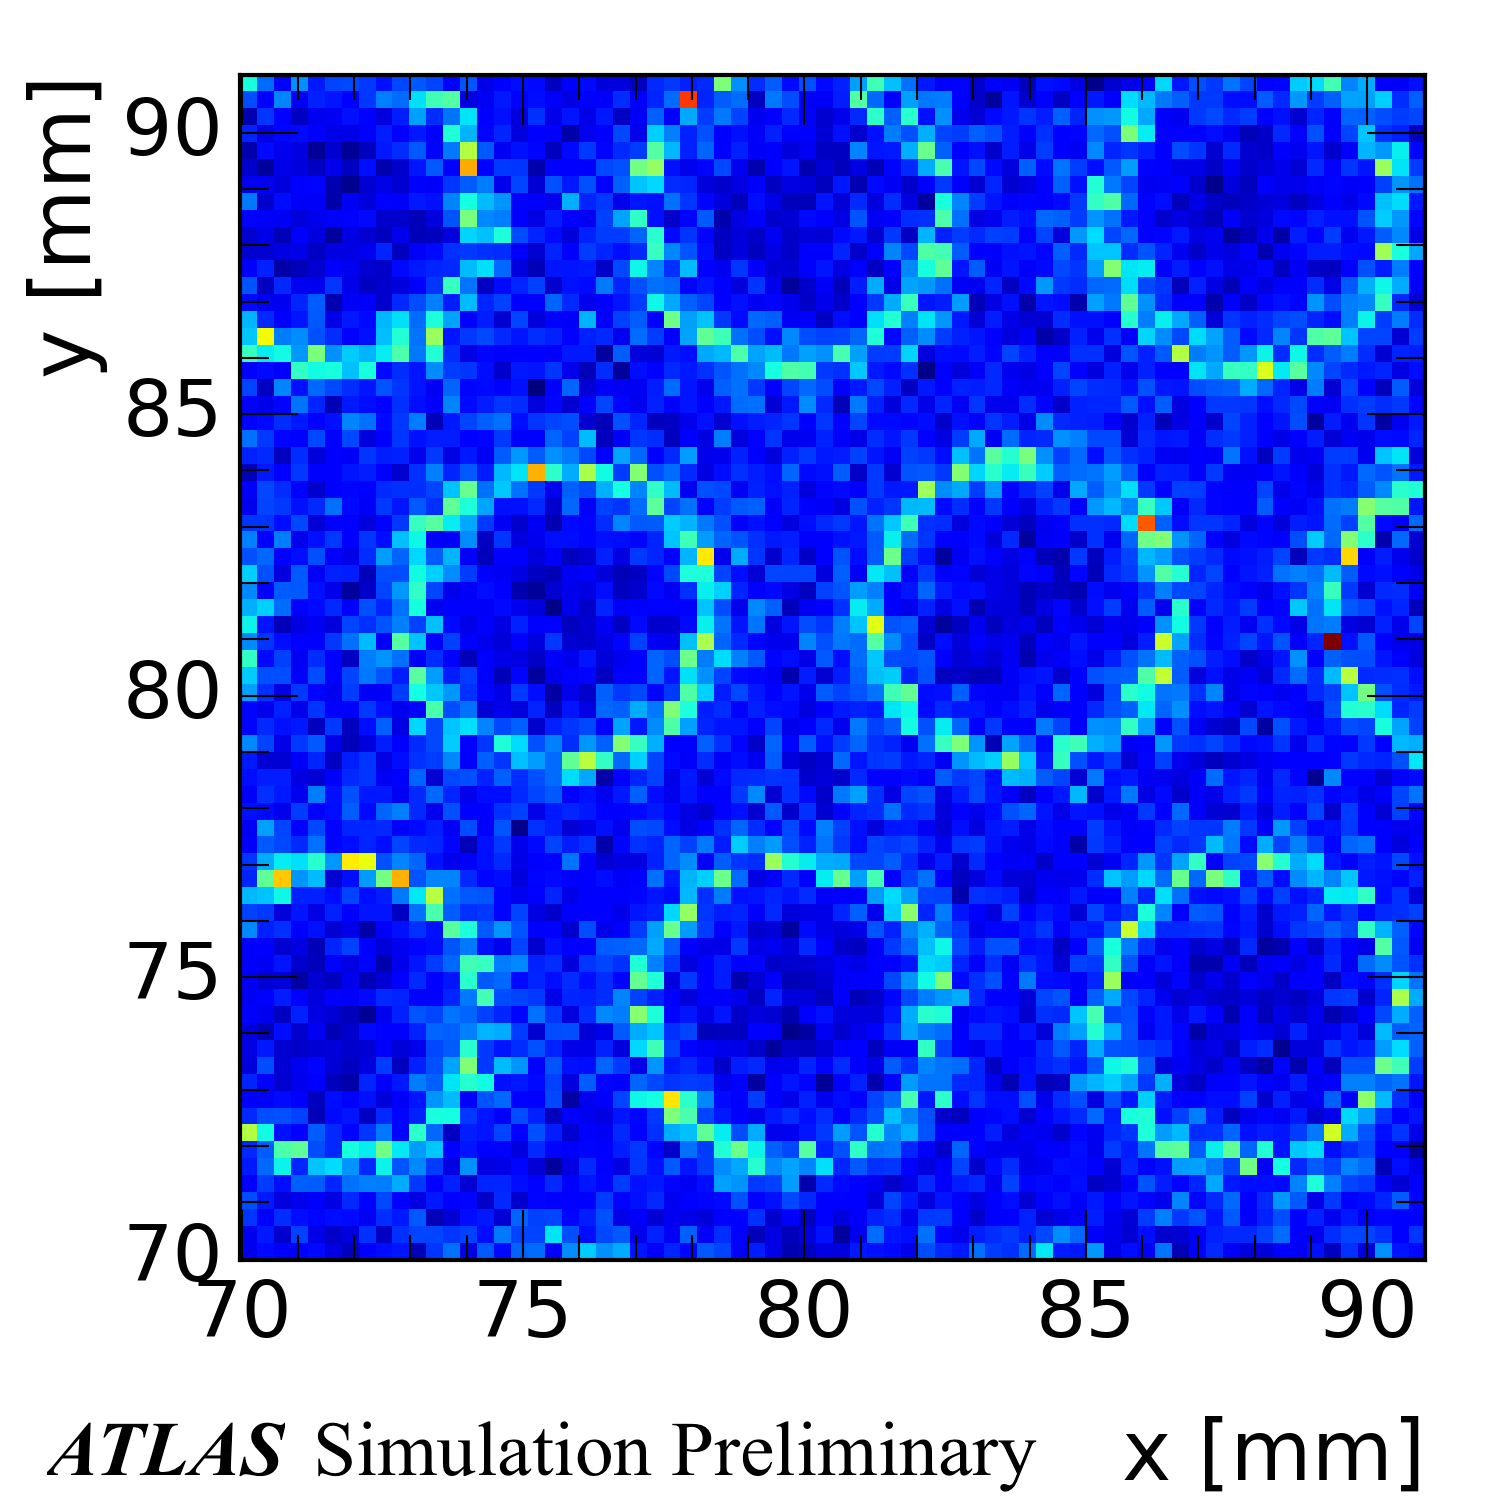
\includegraphics[width=0.5\linewidth]{MC/xySumE.png} }
\caption{Shower energy response histogram in the x vs y plane for electrons, generated with uniformly distributed x and y and energy less than 1 GeV. Light circles are corresponding to a showers, started inside a LAr gaps with on average higher energy response, while the dark parts are corresponding to dead material respectively with smaller sum of the "hits" energy. }
\label{fig:FSFluctuations}
\end{figure}

Fast simulation of forward calorimeters (FCAL) is a complicated task due to its complex structure. As it was mentioned in a Sec. ~\ref{sec:forwardCalo} FCAL consists of hexagonal absorber cells with anode tube and cathod rod in the cell center and liquid argon in the gap between rod and tube. In order to simulate resolution of high energetic electrons, good fast simulation technique should take this feature of large amount of non-uniformly distributed sensitive material.

Resolution of electron inside calorimeter can be written as:
\begin{equation}\label{eq:EMResoultion}
\frac{\sigma}{E} \approx \frac{1}{\sqrt{E}}	\oplus \frac{1}{E} 	\oplus const,
\end{equation}
where symbol $\oplus$ indicates a quadratic sum. The first term is 'stocastic term', which includes intrinsic shower fluctuations, second takes into account readout noise effects and pile-up fluctuations. Constant term derives from non-uniformities in a detector, causing large fluctuation of the energy loss. Resolution of high-energy electrons is mostly dominated by the constant term. 

Fluctuations due to a detector design are visible in a simulation of small energy electrons, generated inside a different points in forward calorimeter. Shower energy $E^{shower}$ distribution in the x vs y plane is showed on Fig. \ref{fig:FSFluctuations}, where shower energy is defined as:
\begin{equation}
E^{shower}=\sum E_i^{hits},
\end{equation}
where $E_i^{hits}$ is an energy of i-th shower deposit inside sensitive material. Periodic structure resembles the calorimeter design, where light circles are corresponding to gaps with liquid argon. It could be reduced to a 1-d problem by introducing distance to a closest rod center. Fig. ~\ref{fig:FSProduction} presents a distribution showers for electrons with energy below 1 GeV coming from initial electrons with energy 1 TeV in the distance to a closest rod center vs shower energy plane. Liquid argon gap is marked by a red lines. There is a clear difference in a showers energies between electrons born in a sensitive and dead material. Difference in a shower properties are also visible for number of hits  (Fig. ~\ref{fig:ShowerProp} a) and standard deviation energy of hits in shower (Fig. ~\ref{fig:ShowerProp} b) distributions. Size of this differences depends on a electron energies and higher for a smaller energies (Fig. ~\ref{fig:FSProduction2} a) and less significant for a higher energies (Fig. ~\ref{fig:FSProduction2} b).  In order to simulate resolution of electrons appropriately , frozen showers method should simulate this distributions close to the nominal. 

\begin{figure}[!tbp]
\center{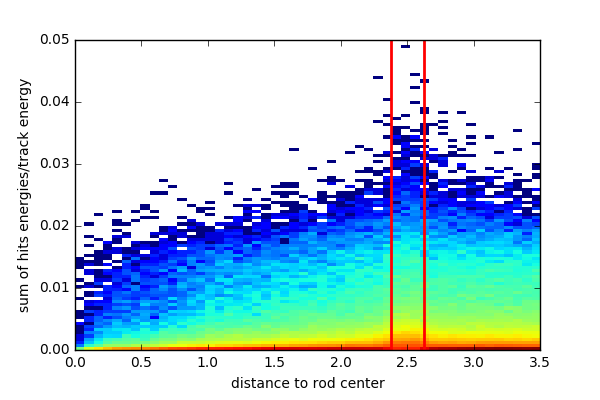
\includegraphics[width=1.\linewidth]{MC/fullBinningScatter.png} }
\caption{Distribution of electron showers for electrons with energy less than 1 GeV coming from initial electron with energy 1 TeV in distance to a closest rod center vs shower energy plane. Position of a liquid argon gap is noted by a red lines. There is visible difference in shower properties between showers inside and outside of the liquid argon gaps}
\label{fig:FSProduction}
\end{figure}

\begin{figure}[!tbp]
\begin{minipage}[h]{0.49\linewidth}
\center{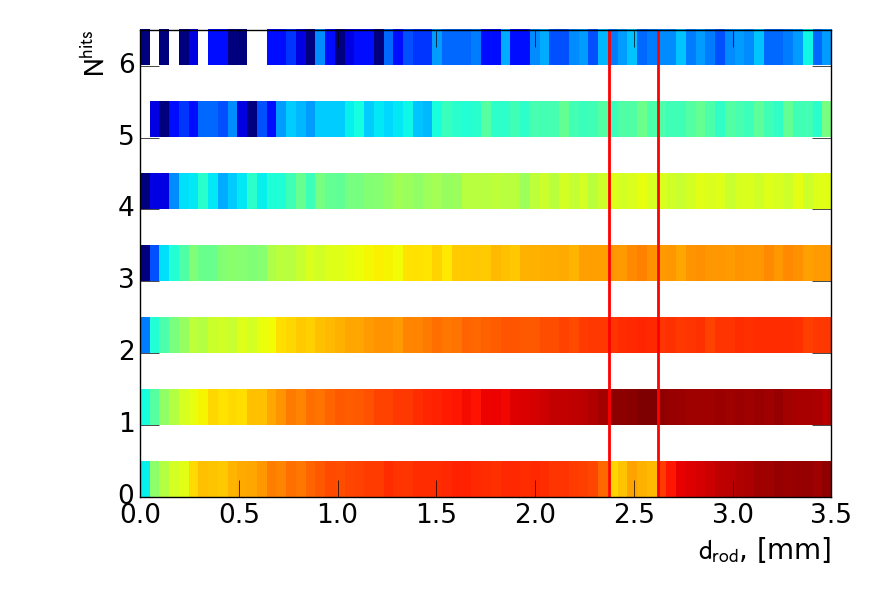
\includegraphics[width=1.0\linewidth]{MC/nHits.png}  \\ a)}
\end{minipage}
\hfill
\begin{minipage}[h]{0.49\linewidth}
\center{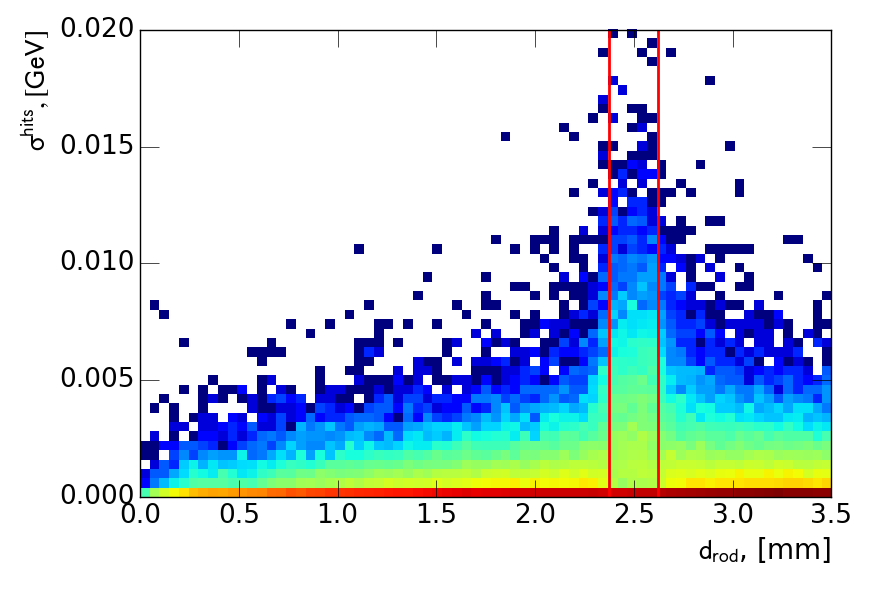
\includegraphics[width=1.0\linewidth]{MC/rms.png} \\ b)}
\end{minipage}
\caption{Distribution of electron showers for electrons with energy less than 1 GeV coming from initial electron with energy 1 TeV in distance to a closest rod center vs a) number of hits in a shower plane and b) standard deviation of hits in a shower energy. Position of a liquid argon gap is noted by a red lines. There is visible difference in shower properties between showers inside and outside of the liquid argon gaps}
\label{fig:ShowerProp}
\end{figure}

\begin{figure}[!tbp]
\begin{minipage}[h]{0.49\linewidth}
\center{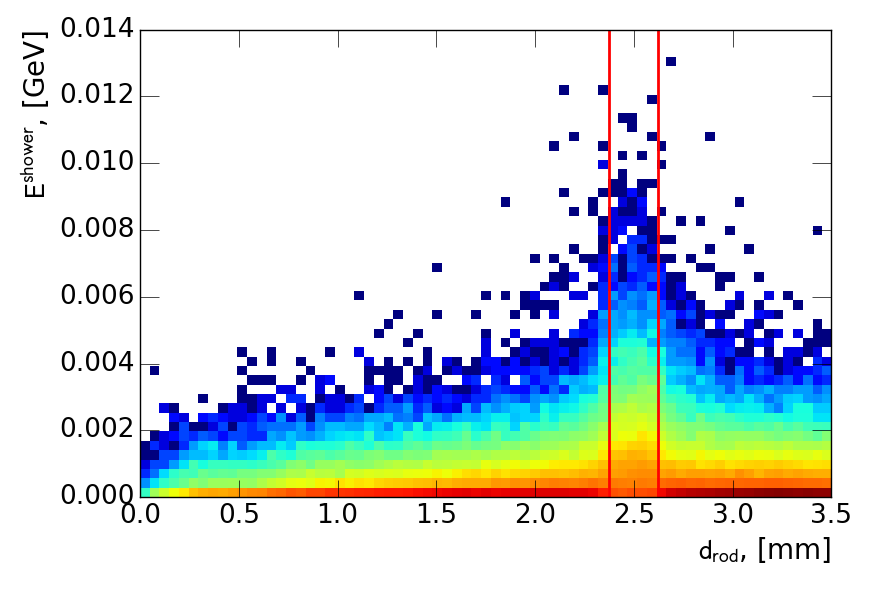
\includegraphics[width=1.\linewidth]{MC/fullBinningScatterSmall.png} \\ a)}
\end{minipage}
\hfill
\begin{minipage}[h]{0.49\linewidth}
\center{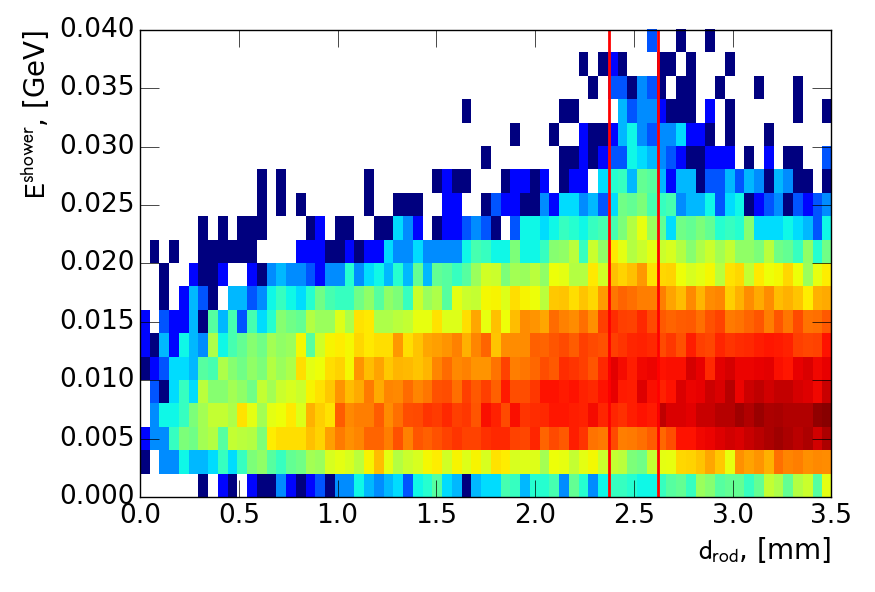
\includegraphics[width=1.\linewidth]{MC/fullBinningScatterBig.png} \\ b)}
\end{minipage}
\caption{Distribution of electron showers for electrons with energy a) less than 100 MeV  and b) higher than 300 GeV coming from initial electron with energy 1 TeV in distance to a closest rod center vs shower energy plane. Position of a liquid argon gap is noted by a red lines. Size of the difference in a shower properties depends on the energy of the electrons and higher for smaller energies}
\label{fig:FSProduction2}
\end{figure}

\section{Frozen showers generation and use in a Monte-Carlo production}

Frozen showers is the main method used in \atlas experiment for a fast simulation of physics inside calorimeter. It replaces a full simulation of a shower with a "frozen" shower from a library. This method consists of 2 stages: library generation and a production use. Because most of the time is spend on a simulation of electromagnetic showers inside froward calorimeters due to their complex structure (Sec. \ref{FCAL}) and a large particle multiplicity, frozen showers are used in simulation of FCAL1 and FCAL2. Main parameters of a frozen shower libraries are summarized in Tab. \ref{tab:MC_FS_params}.

%< Energy have been optimised for something >

 The library itself organized as follows: the header contains basic simulation parameters, like Geant4, geometry and \atlas software release version and physics list used. Showers are stored in a bins of positional  variables (see sec. \ref{sec:FSProd}), while energy remain unbinned. Each shower stores lateral and transverse size and information about energy, time and positions of the hits.
 
During simulation, if an energy of a particle falls below cut-off energy, the particle algorithm examines resulting shower containment. It checks  that particle is far from the edges of calorimeter, so what shower will be by 90\% inside calorimeter. This dependes also on a energy of particle, because shower sizes are growing with energy.
When particle is removed and substituted by shower taken from corresponding eta and distance bin with the closest energy found. Energies of the hits in shower found are scaled to fully correspond to particle energy. Additionally, shower direction is changed to the direction of the particle.

Frozen Showers have been used in \atlas Monte-Carlo production since run-1. This method is applicable for all LAr calorimeters in \atlas, but currently it is enabled for simulation of forward calorimeters (FCAL). 
 
It uses "frozen" showers generated using full simulation.  This showers are stored in a  Particles below minimum energy
thresholds are killed and replaced with with these showers. All of the other particles are simulated using full simulation. This process is schematically shown in a Figure ~\ref{fig:MC_FS_method}.


\begin{figure}[!b]
\center{
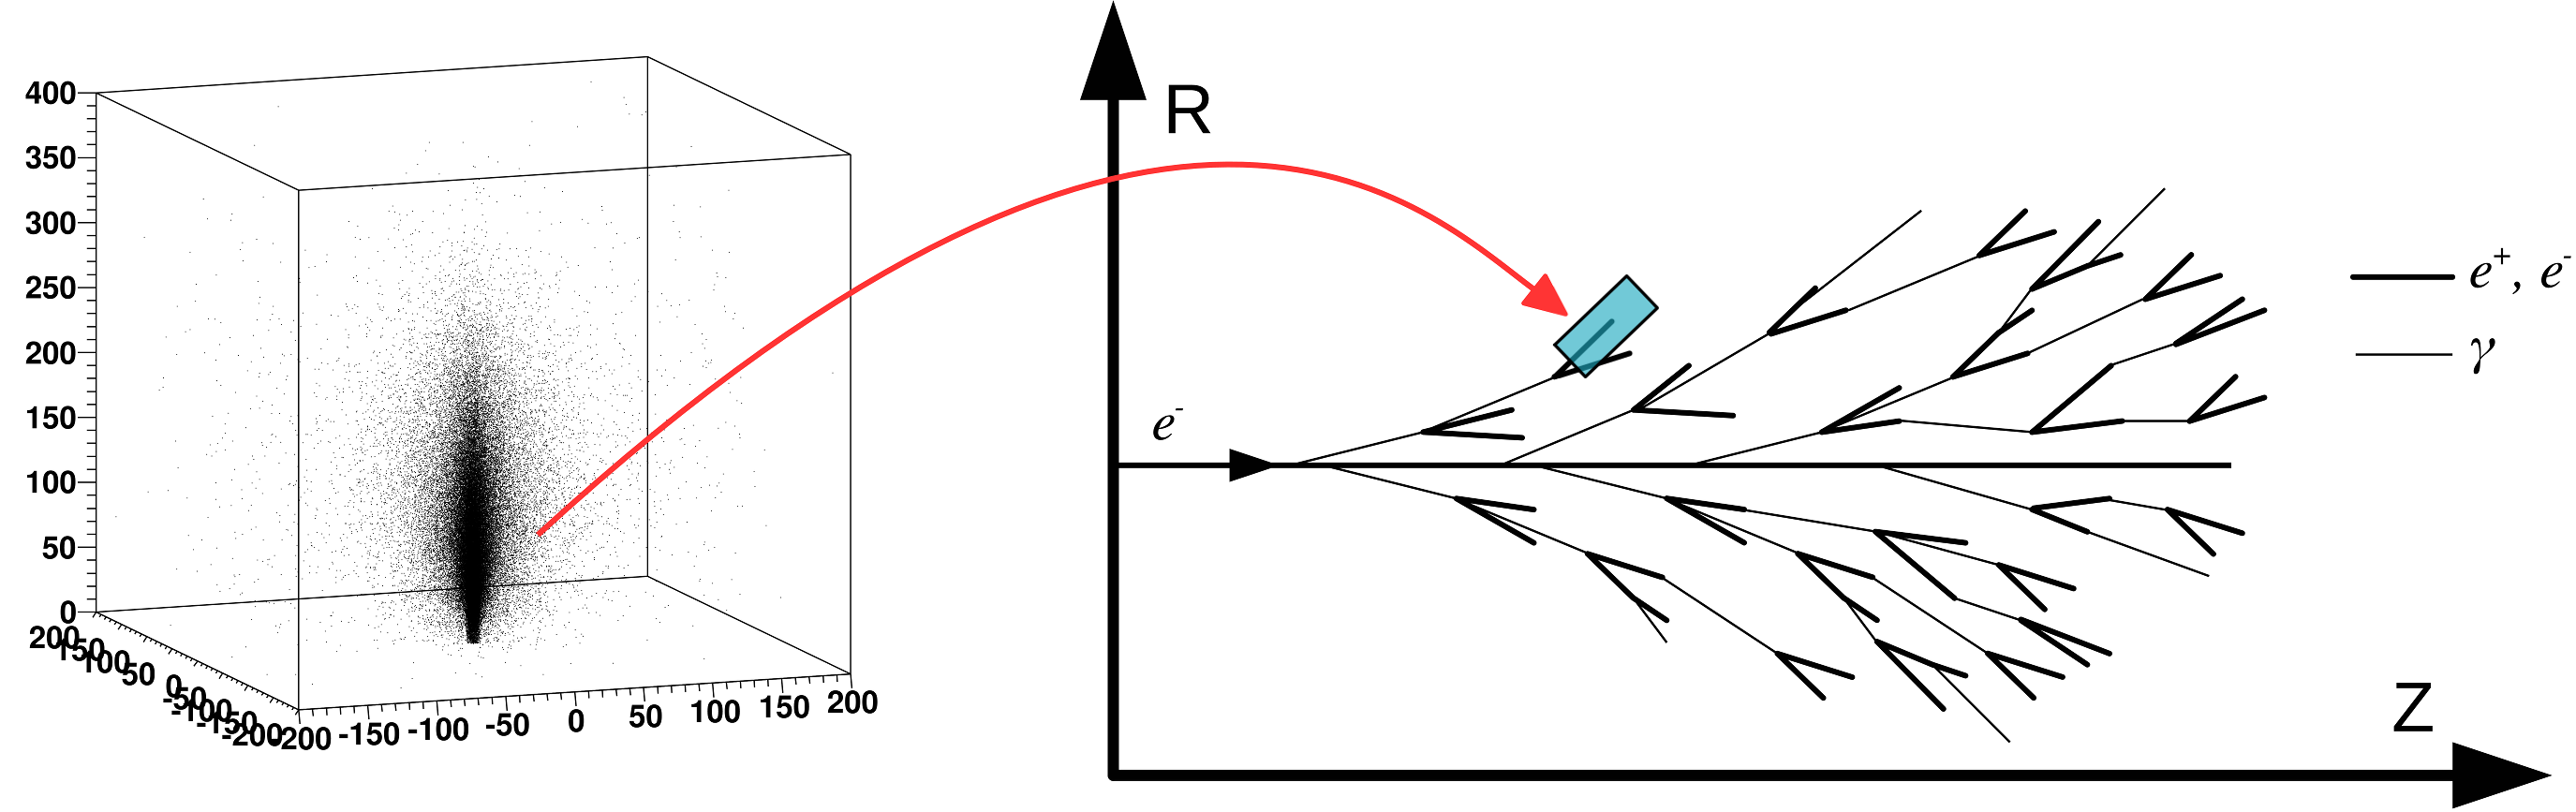
\includegraphics[width=1.0\textwidth]{MC/MC_FS_method.png}
\caption{Diagram showing the shower substitution of the low-energy particle, during the high-energy particle simulation.}
\label{fig:MC_FS_method}}
\end{figure}



\begin{figure}[!tbp]
\center{
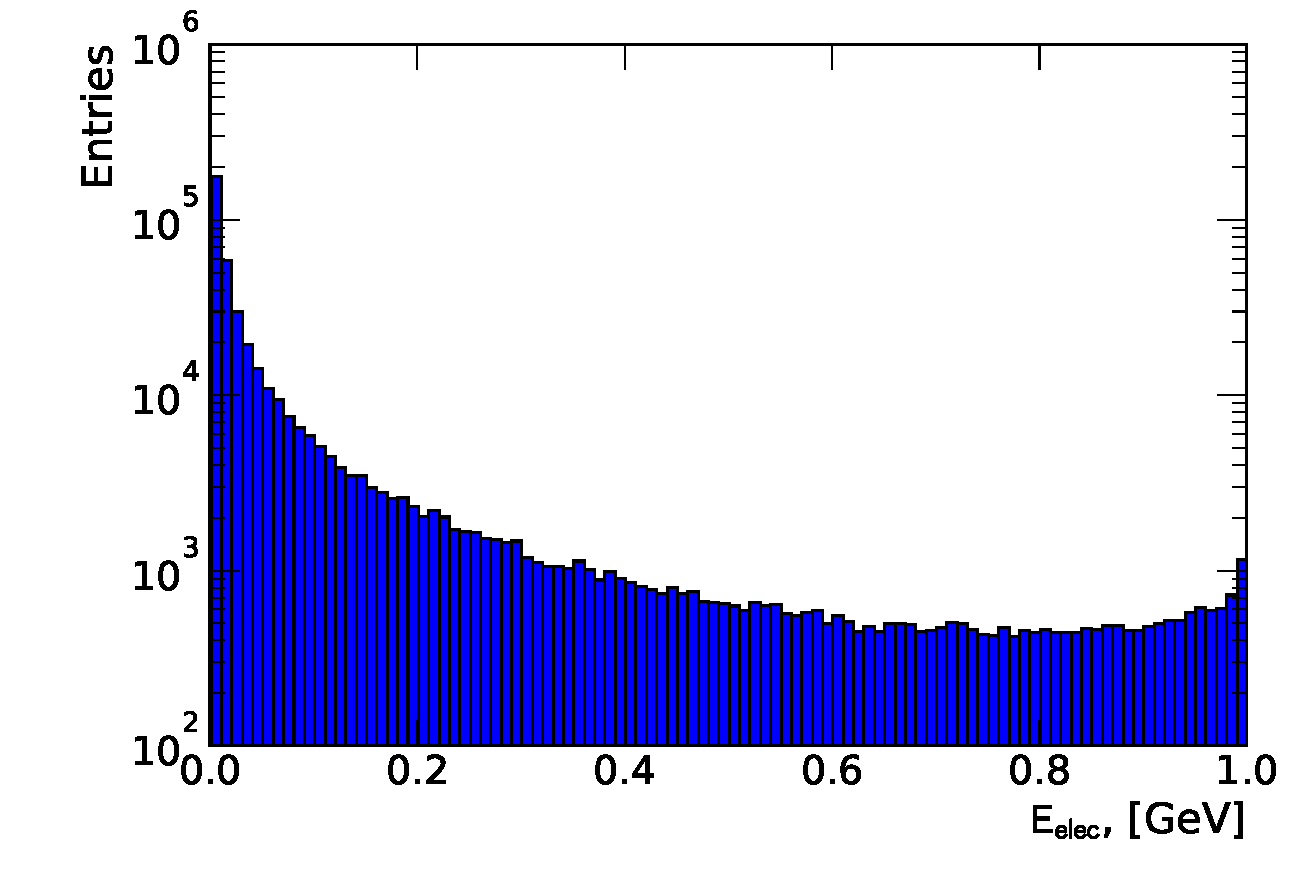
\includegraphics[width=0.8\textwidth]{MC/FSEnergy.pdf}
\caption{Distribution of shower energy used in production of 1000 GeV electrons.}
\label{fig:FSEnergy}}
\end{figure}

Performance of frozen showers is also depending on a lower limit of a method. 
Distribution of shower energies, used for production of high-energetic electron (1000 GeV in that case), is shown on a Figure ~. More than 50\% of them are having energy less than 20 MeV. Studies have showed, that Frozen showers are slower, than a standard Geant4 simulation for showers with energy 3 MeV. This is happening due to library non-binned structure for energy. This makes search of closest energy shower in a library slower, than simulation of shower with zero or one hit in a sensitive detector. 



In a Frozen Shower method there are separate libraries for each particle and subdetector used. Showers should cover fully energy and pseudorapidity region and be able to describe data, that is needed during simulation. This is why 2 stages simulation approach have been used. The first stage takes initial particle parameters from a physical processes (ttbar or a single electron). 

The first stage is to take initial particle parameters, that later will be used in a library from a physical process. This is done using simulation of some process (e.g. ttbar or single electron). Every time, when particle becomes eligible for Frozen Showers, it parameters are saved in a HepMC format. Particles inside calorimeter tend to cluster tightly around initial track, so random truncation of initial particles is used to obtain better detector coverage. On the second stage, this primary particles are propagated through the calorimeter using standart \atlas simulation infrastructure. Resulted shower parameters are saved in a library. This procedure allows to take into account sampling fluctuations and charge-collection effects on a hit information automatically. Additionally, in order to save disc space as well as a memory consumption, hit information is compressed. This compression is done in a two steps, hit merging and truncation:
\begin{itemize}
\item if the distance between any two hits is smaller, than a given parameter $R_{min}$, then hits are merged into one deposit at the energy weighted center of them. This process is done iterativelly.
\item hits whose energies are below the fraction f of the total energy sum of all hits, are truncated. The energy of remaining hits is rescaled back to preserve the total deposited energy.
\end{itemize}

Unfortunately, for a Frozen Showers, generated for Run-1 monte-carlo, additional tuning of electron libraries was needed. This was done using reconstructed energy of electrons. Frozen Showers tend to underestimate fluctuations of energy loss, that is leading to a smaller electron resolution for a high energies. Correction is done by enlarging bin, corresponding to a gap position. Also, correction of the mean shift is done by scaling energy response of all showers. After this frozen showers are showing good agreement with full simulation. This procedure needs to be done every time, when something is changing in software. Because tuning is done manually, lots of a manpower is needed for each Monte Carlo mass production campaign.



\begin{figure}[!tbp]
\center{
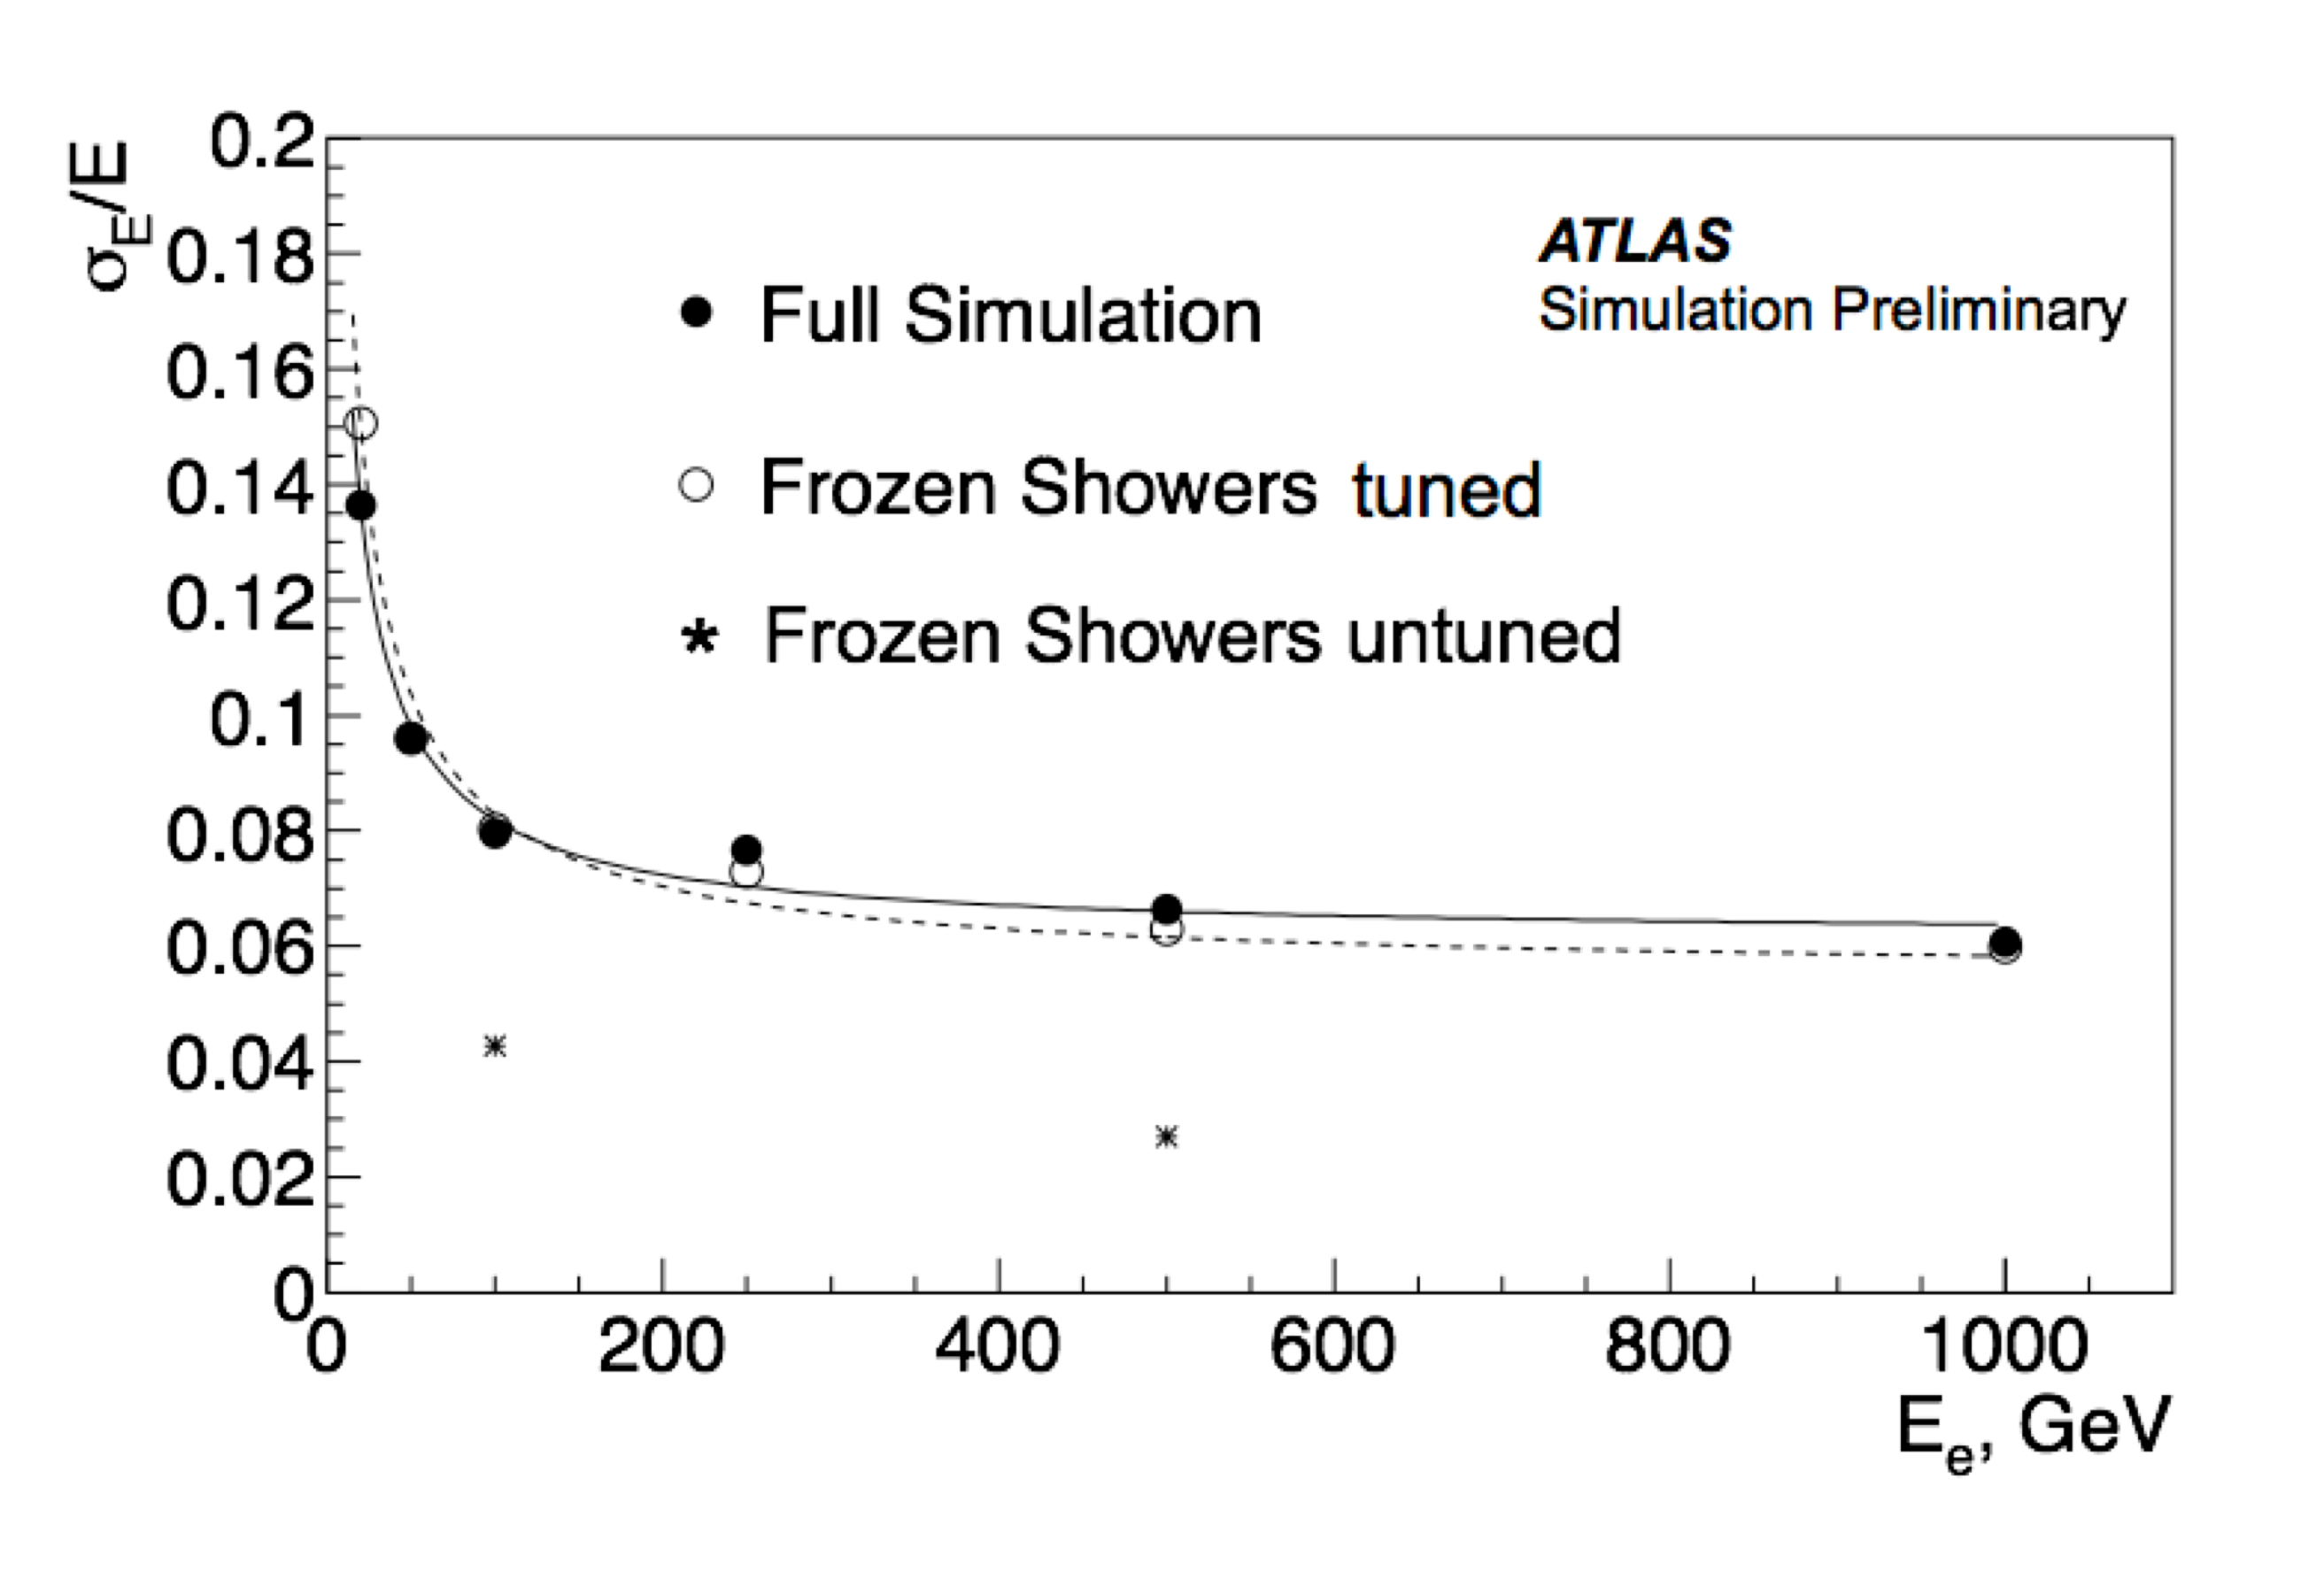
\includegraphics[width=0.7\textwidth]{MC/fs.png}
\caption{Electron resolution for full simulation, tuned and untuned frozen showers}
\label{fig:FS_resolution}}
\end{figure}
\section{Library generation}
\section{Use of Frozen Showers in MC production}

\section{Tuning of Frozen Showers libraries}
As it was mentioned before, process of library generation can be comlicated and take a lot of the time because of the needed tuning. In this subchapter possible ways to improve frozen showers performance have been studied. 
\begin{figure}
\center{
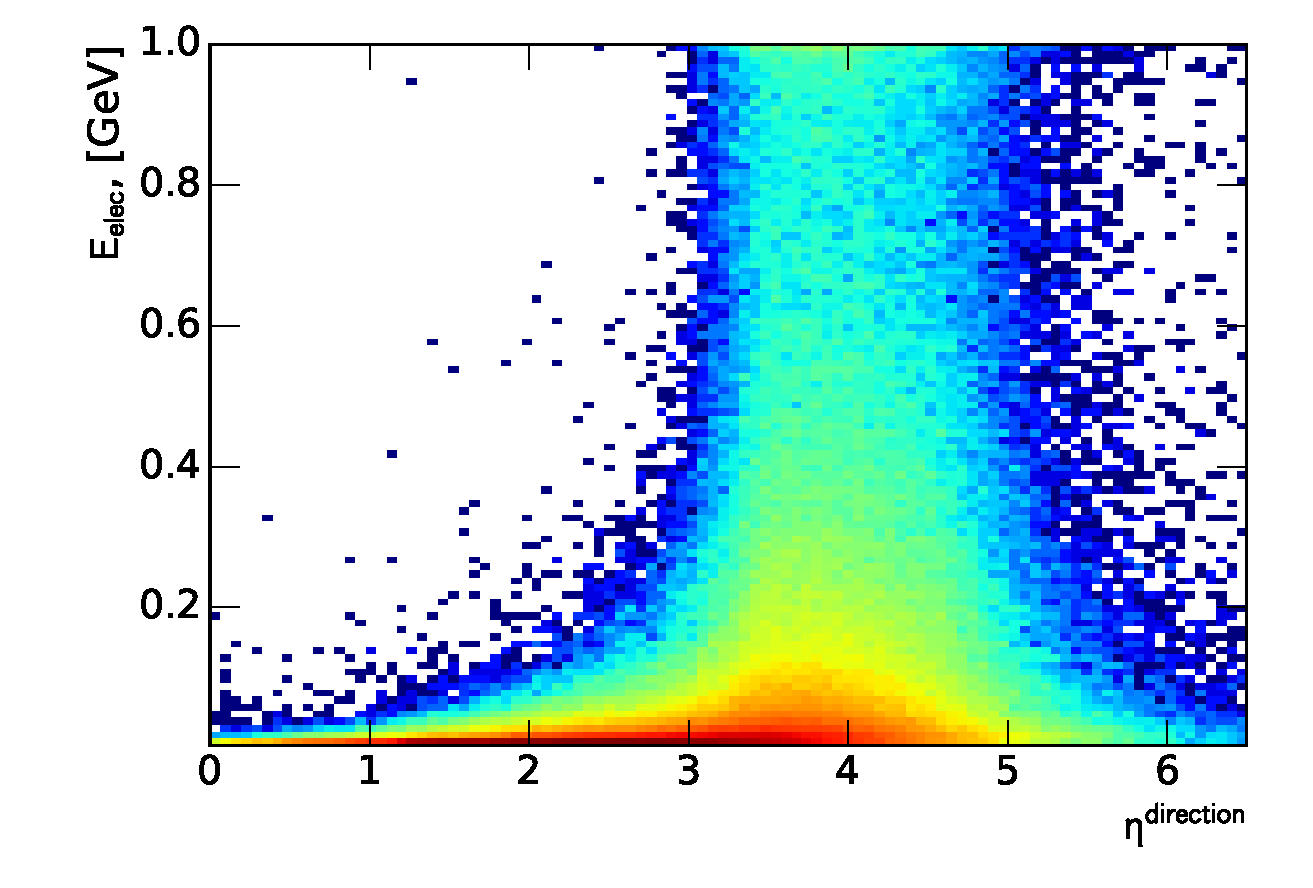
\includegraphics[width=0.8\textwidth]{MC/FSEtaMomVsEnergy.pdf}
\caption{Distribution of showers used in production of 1000 GeV electrons on shower energy vs $\eta_{momentum}$ plane.}
\label{fig:EtaMomVsEnergy}}
\end{figure}

As it was mentioned before, that there are two type of material used in a FCAL. Showers within them are giving different response, what is affecting overall reconstructed electron energy resolution.  At the first generations distance bin have been corresponding to LAr gap or dead material positions. During tuning bin with LAr was enlarged to gain a better agreement with full simulation. So, one of the basic ideas to improve frozen showers performance is to change a size of LAr gap in a library generation. 

It was decided to treat showers, that have been born near LAr gap and crossed it on a radiation length, in a same way with showers in sensitive material gap, and call them sensitive material showers. Oppositely, showers, that haven't crossed LAr gap, are called dead showers. This model leads to a bigger gap width by a definition. One of the possible ways to find this bin position automatically is to use machine learning tools. 

Machine Learning is a set of algorithms, what allows computers to learn and give a predictions without being specifically programmed. This is a modern field of computer science, that is wildly used in a different fields like computer vision, natural language processing, data science etc. There are two main types of machine learning algorithms: supervised, where example of desired output is given by the "teacher" and the goal is to learn a general rule, that maps inputs to outputs and unsupervised learning, then there are no labels given to algorithm, and algorithms is discovering hidden patterns in data. Initial data parameters of interest, that are used in algorithm to learn are called features. It is important to have right proper set of features and good training sample. 

From a geometrical point of view, one of the main parameter is a direction of the shower. Eta momentum distribution is showed on a Figure ~\ref{fig:EtaMomVsEnergy} . Most of the showers are collinear to an electron direction. Because of this it was decided to use as a training sample simulation results for electrons with energies less than 1 GeV and momentum uniformly distributed between eta 3.0 and 4.0. This allowing to study equally low and high energy showers equally.

\begin{figure}[!tbp]
\begin{minipage}[h]{0.49\linewidth}
\center{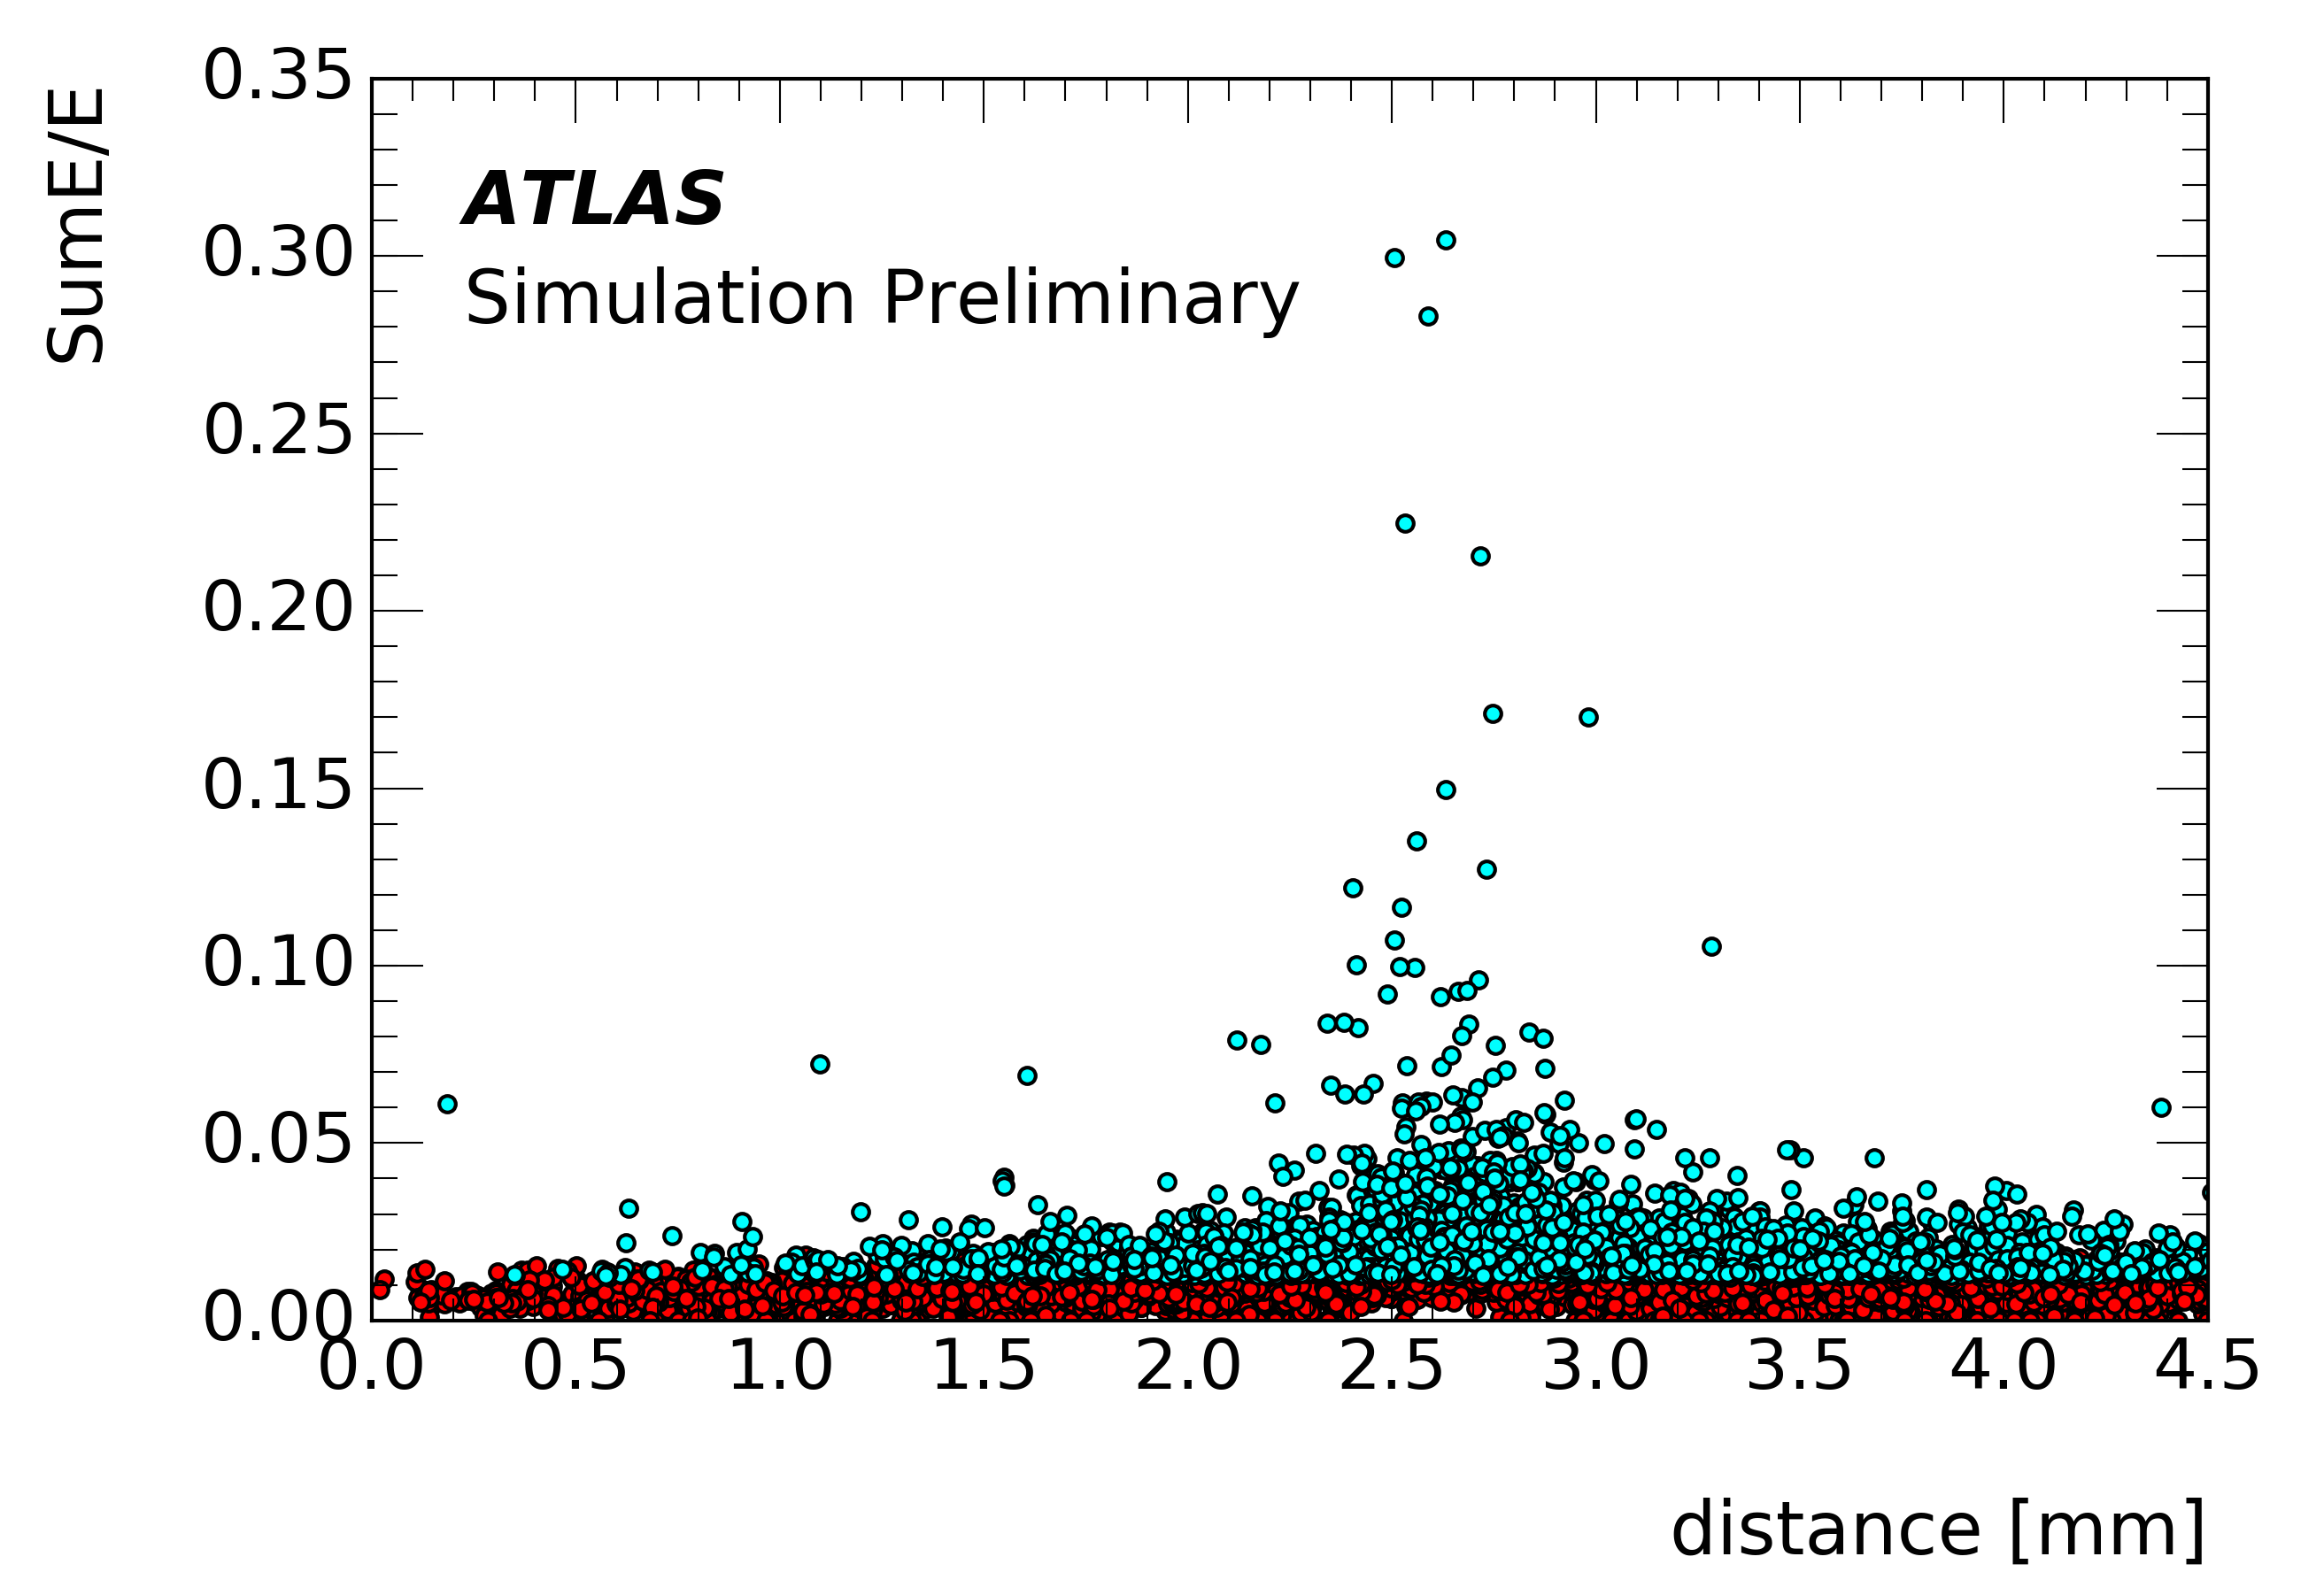
\includegraphics[width=1.\linewidth]{MC/firstClassifier.png} \\ a)}
\end{minipage}
\hfill
\begin{minipage}[h]{0.49\linewidth}
\center{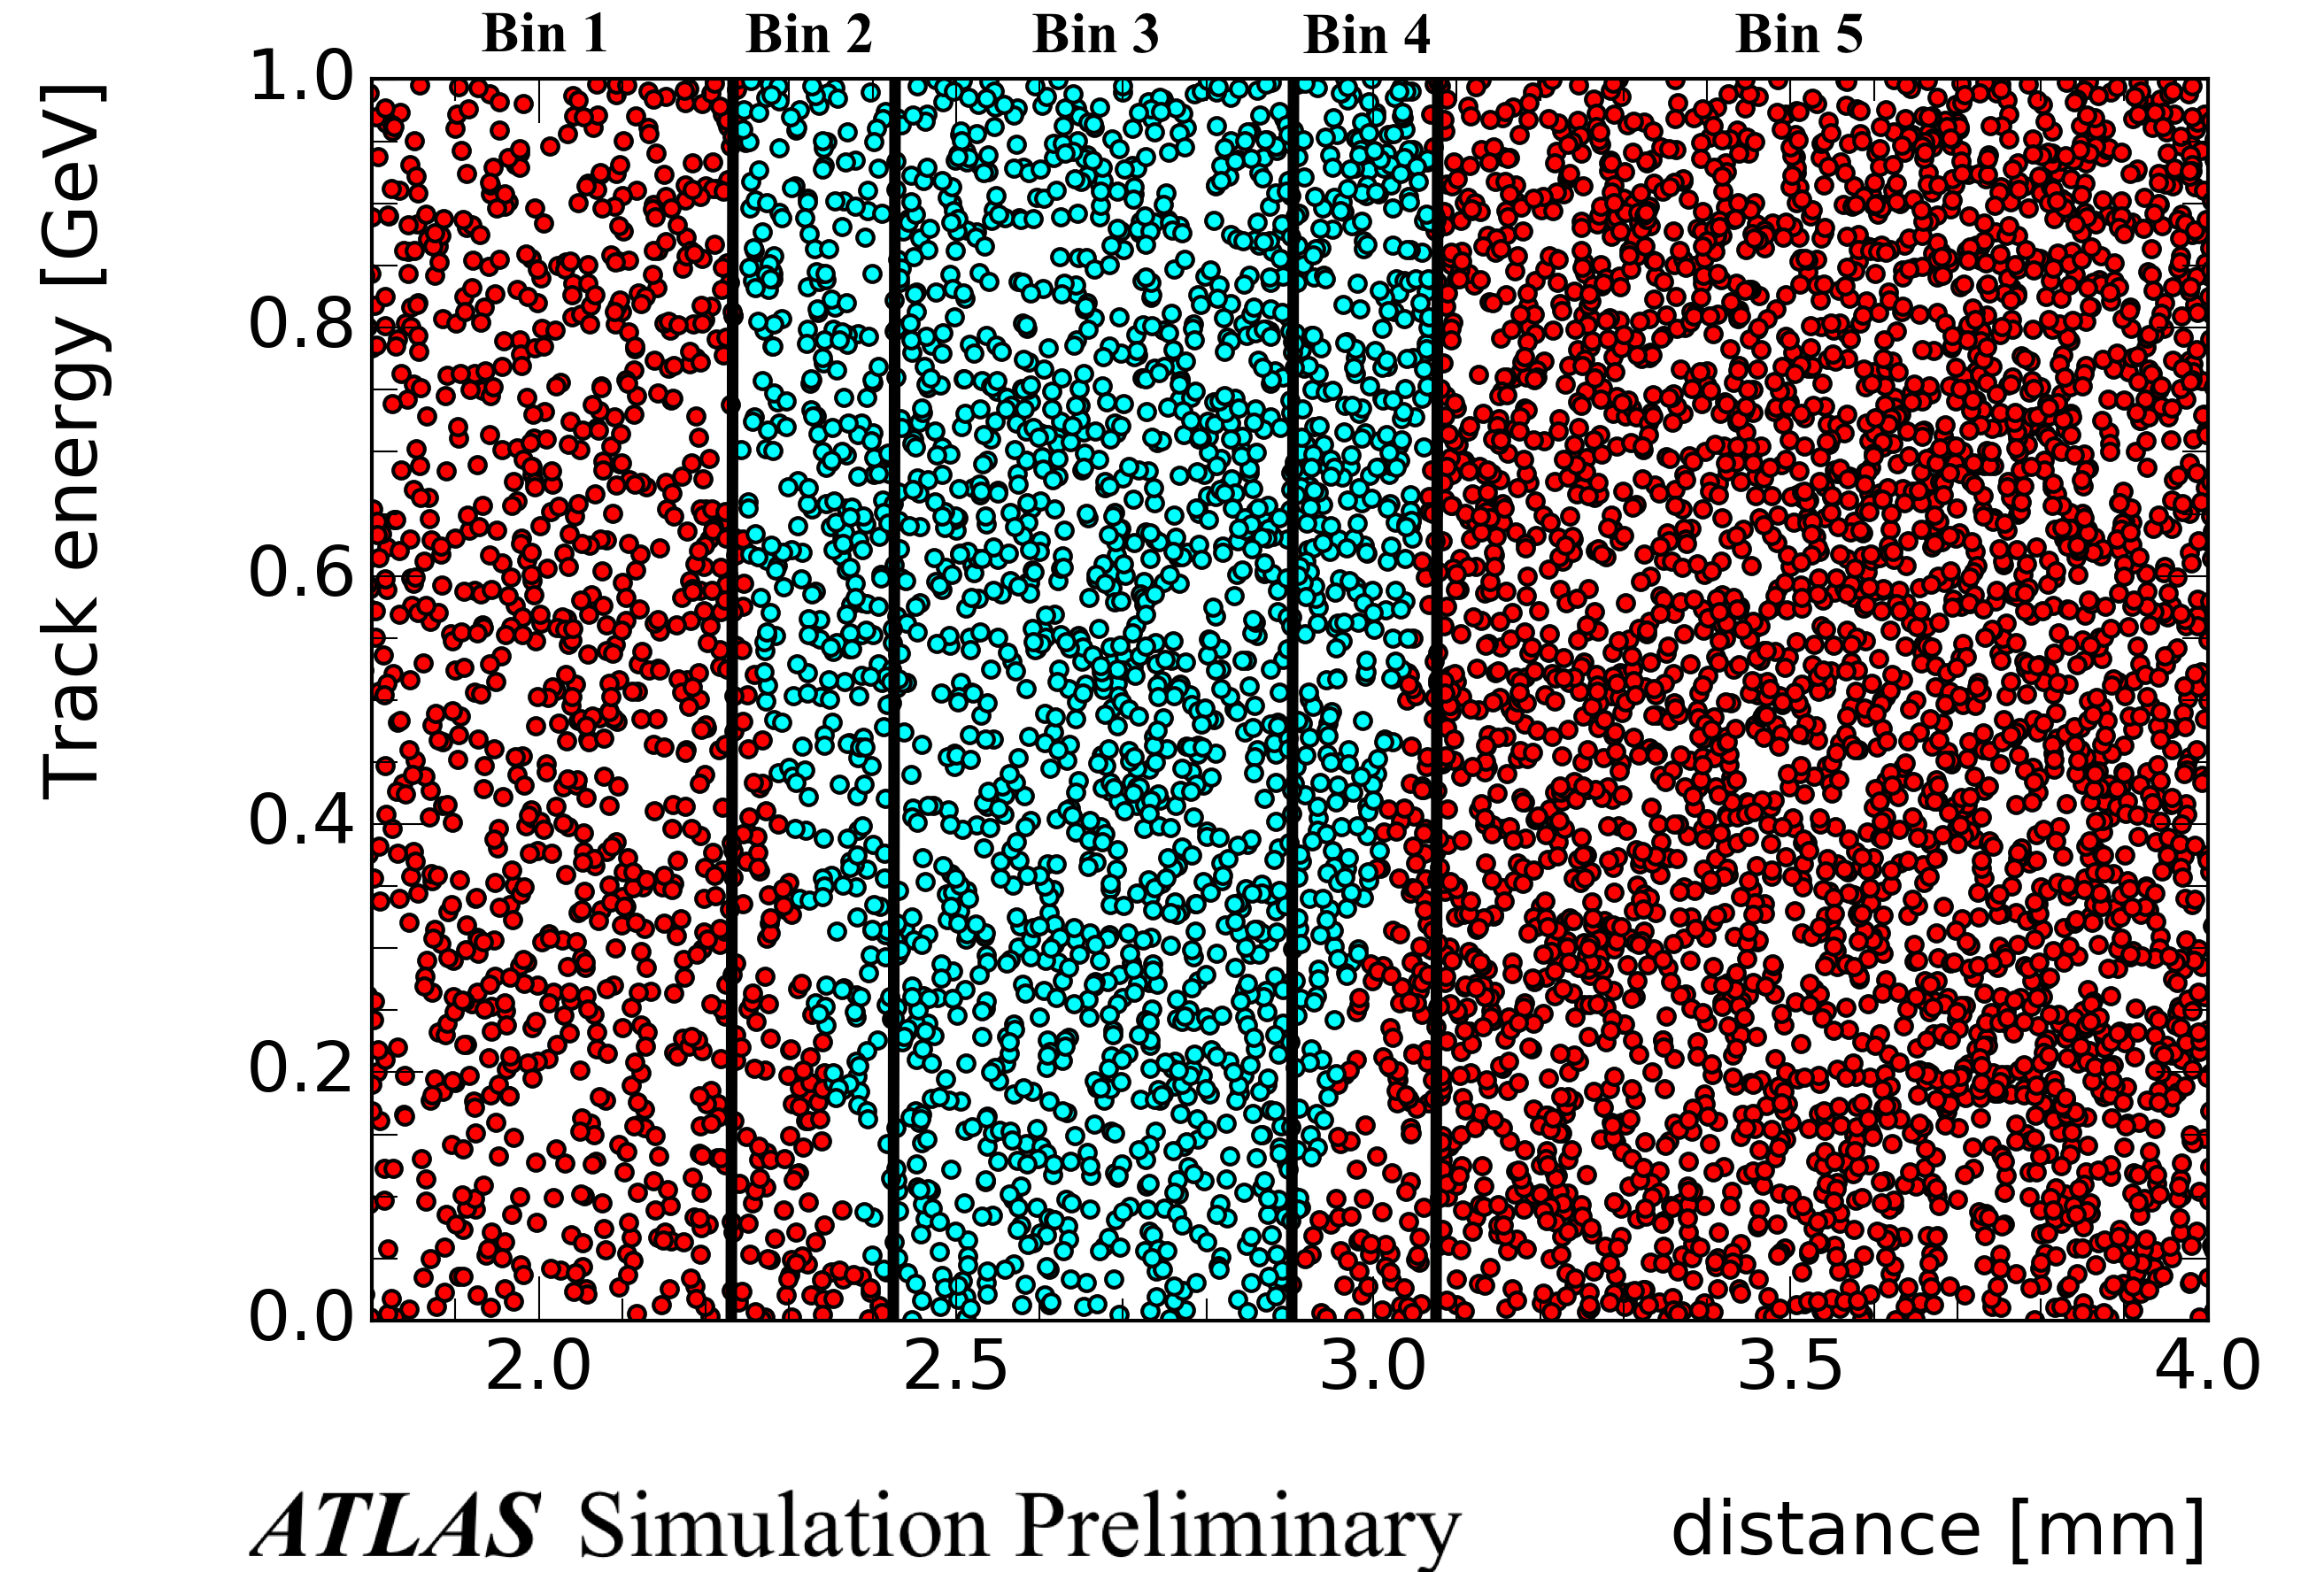
\includegraphics[width=1.\linewidth]{MC/secondClassifier.png} \\ b)}
\end{minipage}
\caption{Results of machine learning for a) first classifier b) second classifier. Cyan dots are corresponding to sensitive material showers, red - dead material showers}
\label{fig:Class}
\end{figure}


From out definition of 2 classes of showers, it is simple to construct a pre-labelled training sample. This is done by reducing initial sample and taking showers near rod center and inside liquid argon gap. Output of this classifier, that was trained on with sample with shower features, such as energy response and number of hits, than can be used to expand our labels to a full distance range. Than it can be used as an input to a second classifier, which will separate two types of showers using particle parameters, such as energy and distance to a rod center. For a first step decision trees have showed good classification efficiency (around 97\%). For a second classifier support vector machines have been used. This method is trying to reconstruct a hyperplane, that is dividing two classes. Outputs of both of this classifiers are shown on a figure . New gap position is determined using borders of hyperplane. This procedure is giving expected from the initial model results. Gap is wider, than and original one. It is also getting bigger with bigger energy, because of the radiation length growth. 
Validation results for two different eta bins are shown on figure ~ a) and b). In a bin this new binning is performing better, than original one without any additional tuning. Unfortunately this is not true for all of the bins, as we can see on a figure ~ b). This eta bin have showed worst performance for a new binning, but it is performing still better, than original binning without tuning.

\begin{figure}[!tbp]
\begin{minipage}[h]{0.49\linewidth}
\center{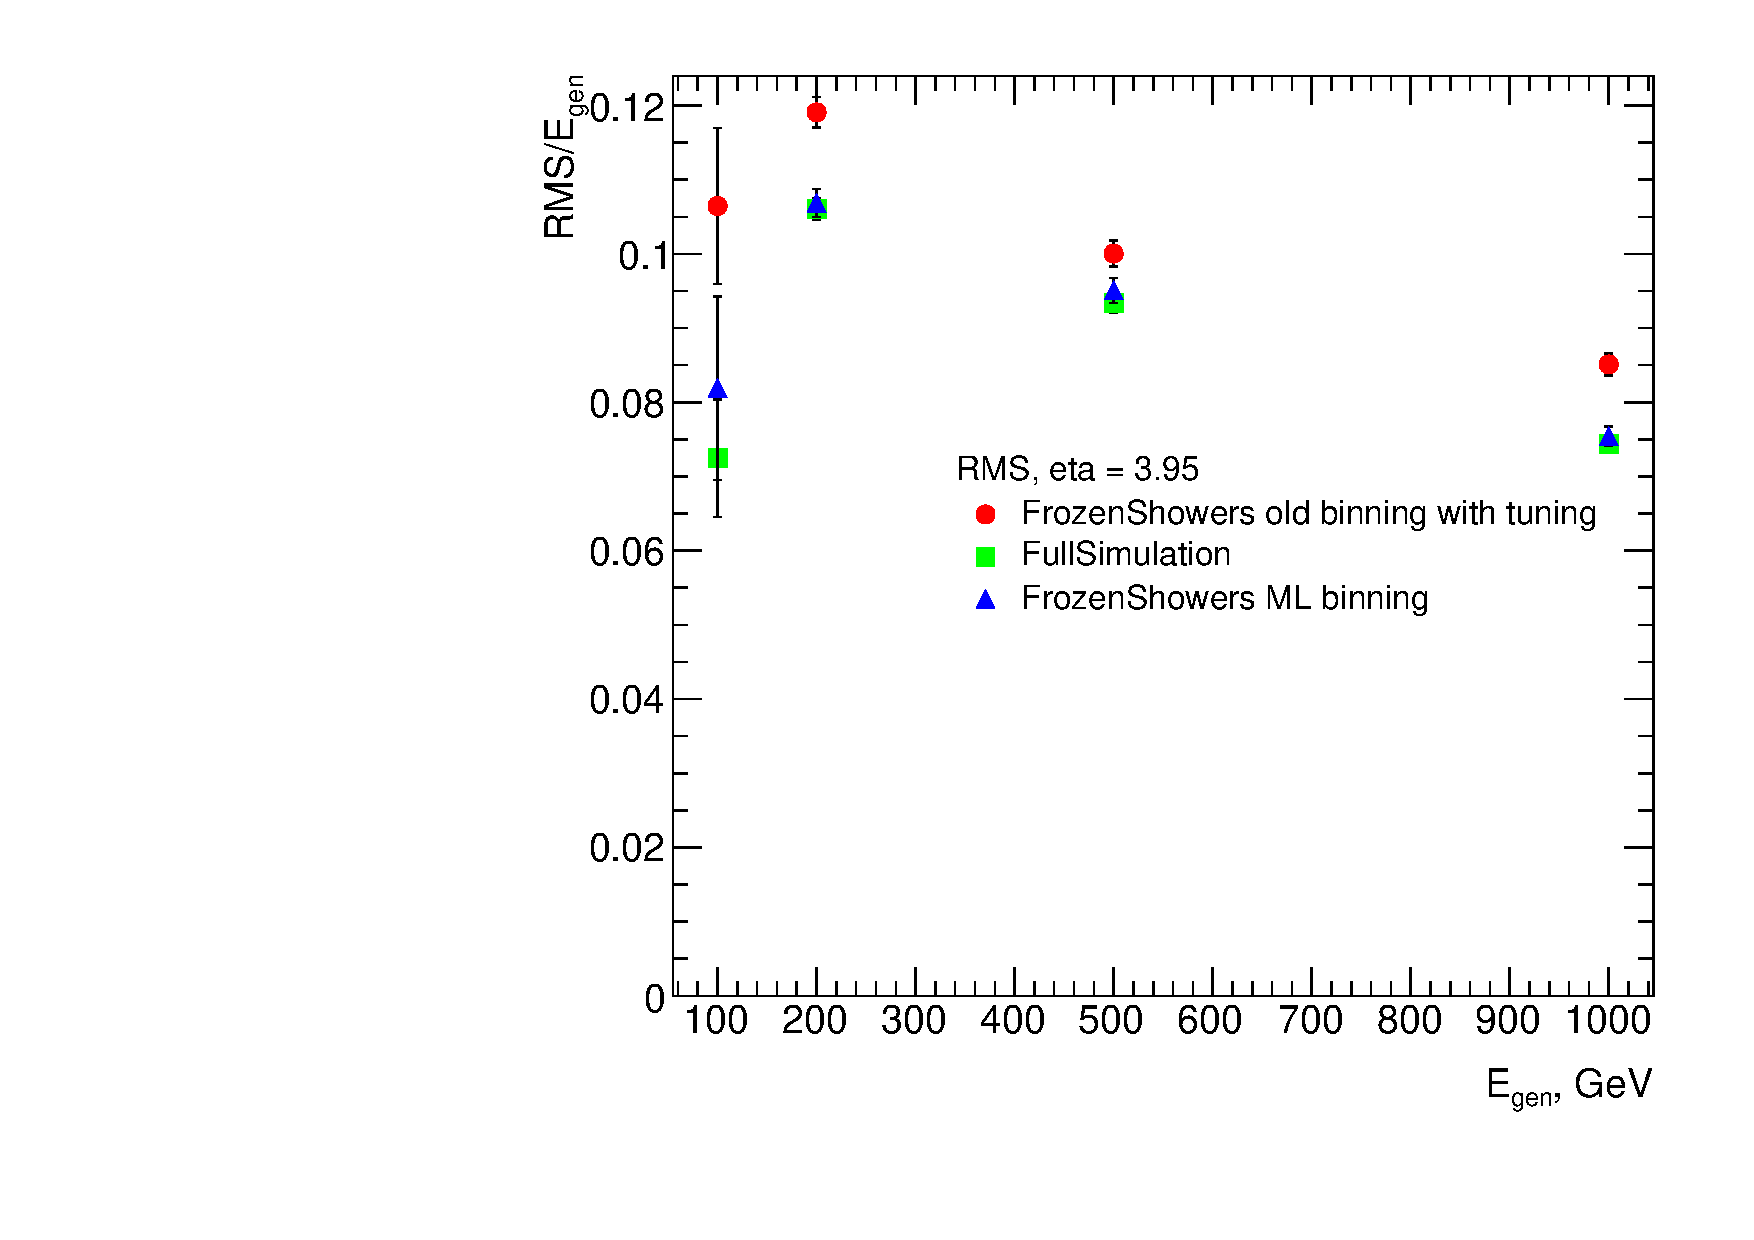
\includegraphics[width=1.\linewidth]{MC/rms3p95.pdf} \\ a)}
\end{minipage}
\hfill
\begin{minipage}[h]{0.49\linewidth}
\center{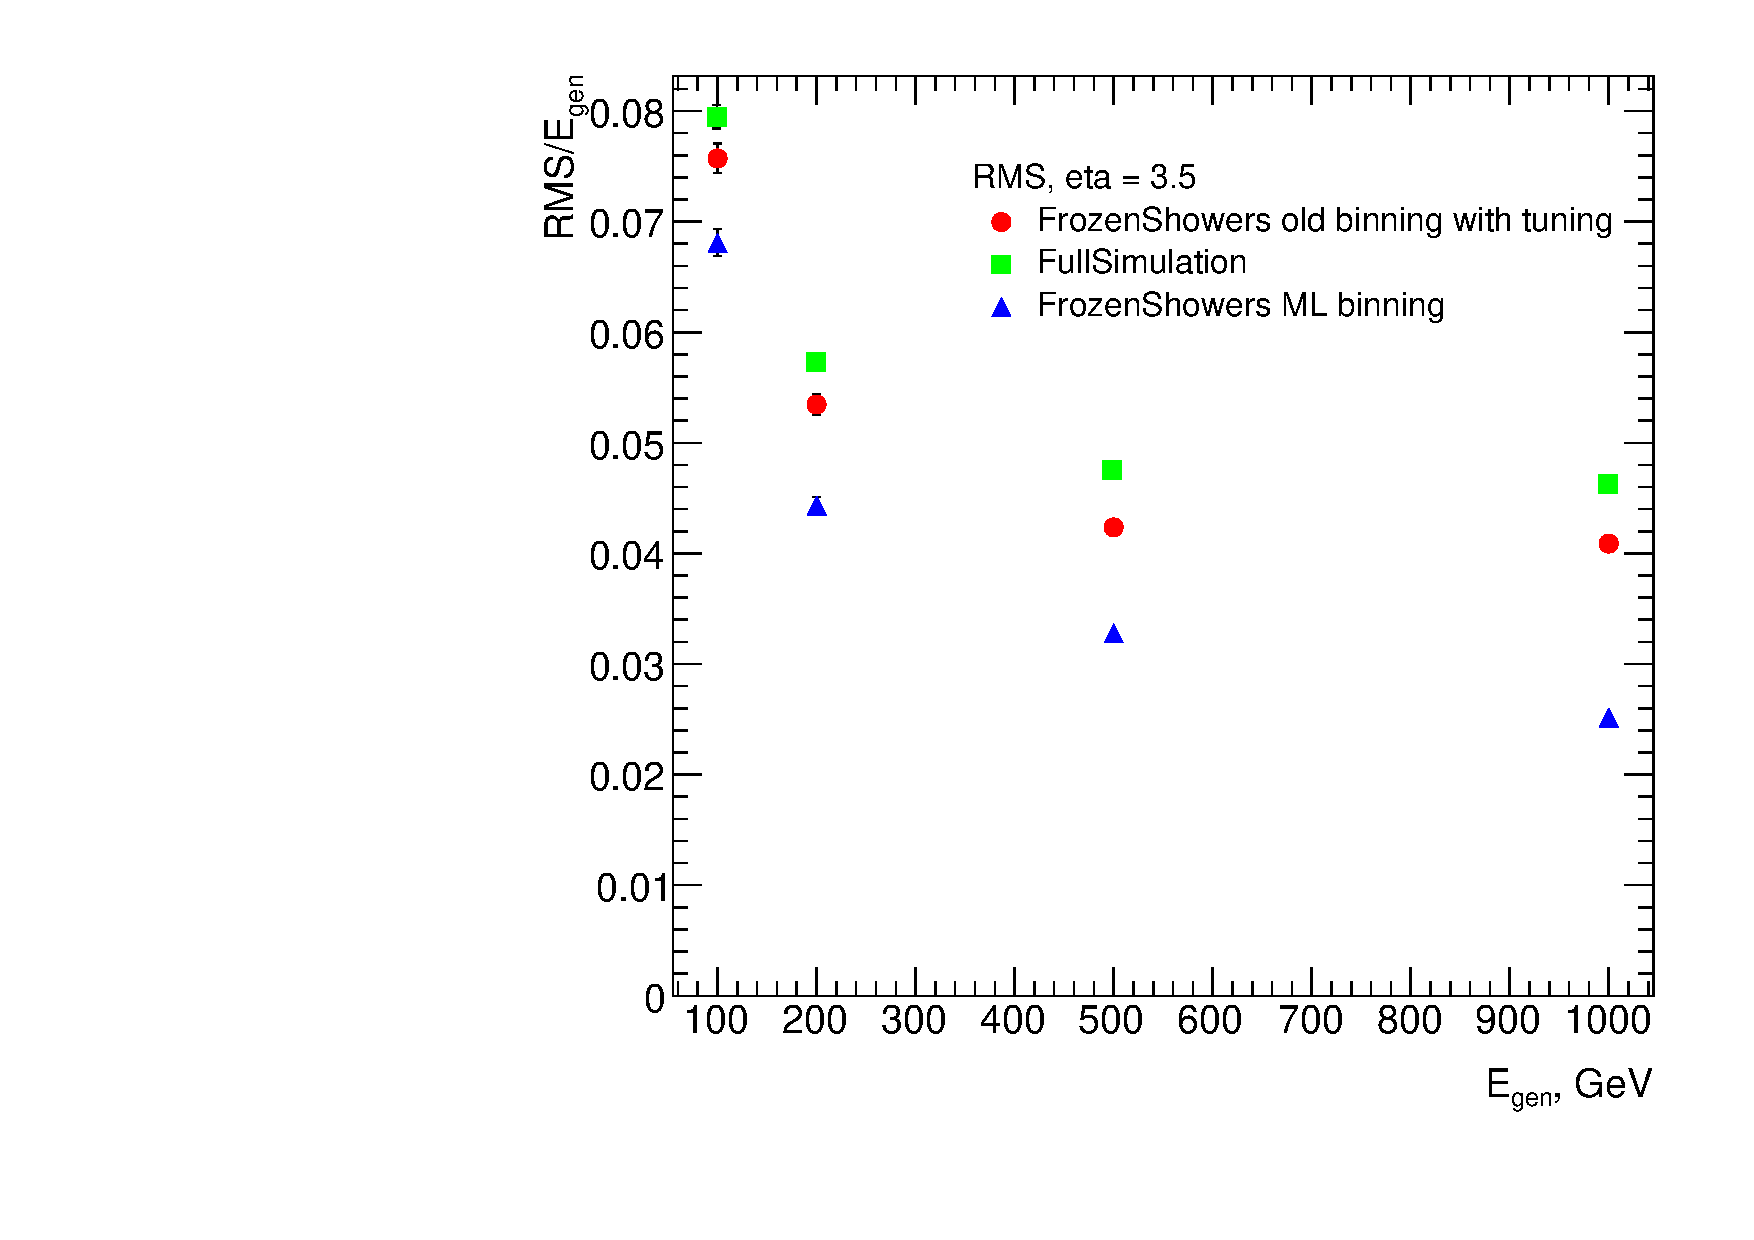
\includegraphics[width=1.\linewidth]{MC/rms3p5.pdf} \\ b)}
\end{minipage}
\caption{Resolution of reconstructed electrons for full simulation, new libraries with ML binning and old tuned libraries with original binning for a) eta =3.95 b)eta=3.5 }
\label{fig:Class}
\end{figure}

This binning was used in a production of new libraries for Monte Carlo in a Run-2. It is planned to use more precise training sample for a future iterations of this procedure for improving performance of outlying eta bins.

\section{Validation of the new libraries}
\section{Plans for a future}